\section{iBox (Ultra-compact Fanless Embedded Computer)}
\subsection{Définition et Rôle des iBox} 
Les iBox sont des ordinateurs embarqués ultra-compacts et sans ventilateur, spécialement conçus pour des applications industrielles nécessitant fiabilité et robustesse. Ces dispositifs jouent un rôle crucial dans la collecte et le traitement des données des automates.
\subsection{Caractéristiques principales de la série 5000 des Embedded Box PC}

\begin{figure}[H]
    \centering
    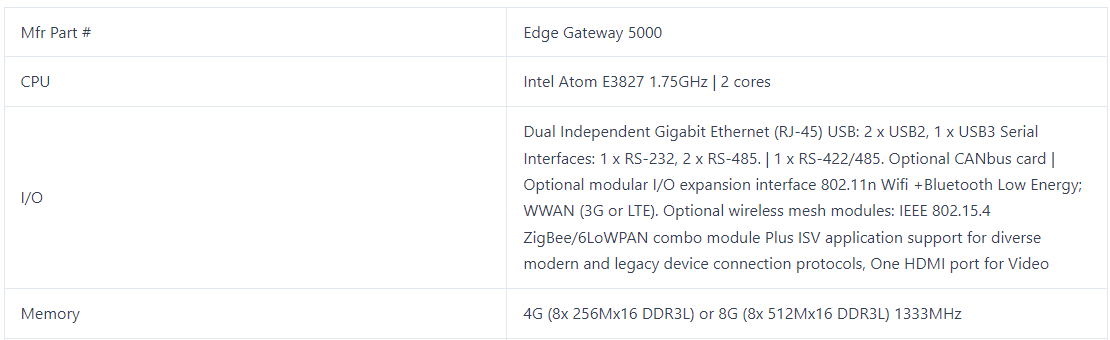
\includegraphics[width=1.1\textwidth]{chapters/5/img/DELLLL.png}
    \caption{Dell Embedded Systems Featuring Intel Atom E3800 Processors}
    \label{fig:campus}
\end{figure}

\subsection{Caractéristiques principales des iBox :}

Compact et Fanless : Conception sans ventilateur, réduisant les risques de défaillance mécanique.
Performance : Capables de traiter des volumes de données importants en temps réel.
Connectivité : Équipés de multiples interfaces pour faciliter la communication avec divers systèmes.
\subsubsection{Applications typiques :}
\begin{itemize}
    \item  Industrial automation involves process control and supervision.
    \item  Fleet monitoring and management, including real-time data collecting and processing. Collecte et traitement des données en temps réel pour une gestion optimisée.
    \item IoT and Edge Computing solutions: Analyze data locally before sending it to a data center or cloud.
\end{itemize}


\section{Test de connectiviter via mqtt }7